\section{Messaufbau}
Damit die verschiedenen simulierten Ansteuerungsarten in der Praxis umgesetzt werden können, wurde ein Messaufbau aufgebaut. In diesem Kapitel sind alle Komponenten, welche für den Messaufbau benötigt wurden, aufgeführt. Dazu gehören die Spannungsverstärkerschaltung, welcher sich auf dem Arduino befindet, das eingebaute Filter sowie der Arduino selber, der für die verschiedenen Funktionen programmiert wurde.
\subsection{Laboraufbau}
Die Praxistests wurden mit einem \grqq T-Drive 3Ph compact Thyristorsteller\grqq \hspace{0.02cm} von der Firma Chemtronic durchgeführt. Wie der Name des Produktes sagt, arbeitet diese Thyristorschaltung mit drei Phasen. Für die Ansteuerung des Zündwinkels kann ein Potenziometer verwendet werden. Dies hat jedoch den Nachteil, dass der Zündwinkel von Hand eingestellt werden muss. Jedoch kann für die Ansteuerung auch ein Spannungssignal von 0 - \SI{10}{V} benutzt werden. Dieses Spannungssignal entspricht linear dem Zündwinkel 180\textdegree \hspace{0.02cm} bis 0\textdegree \hspace{0.02cm} der Thyristoren. Um dieses Spannungssignal erzeugen zu können, wurde ein Arduino Mega 2560 verwendet. Er erzeugt jedoch nur eine Ausgangsspannung von \SI{5}{V}. Deshalb wurde eine Spannungsverstärkungsschaltung entworfen, die die Spannung verdoppelt. Die PWM-Funktion im Arduino konnte genutzt werden, damit die Spannung variabel bleibt. Das PWM-Signal läuft mit einer Frequenz von \SI{490}{Hz} \cite{Arduino_PWM}. 
Damit der Operationsverstärker der Verstärkungsschaltung die Spannung richtig verstärkt, muss zwingend ein reines DC-Signal am Eingang des Operationsverstärkers anliegen. Deshalb wurde zusätzlich ein Tiefpass-Filter erster Ordnung am Ausgang des Arduinos eingebaut, mit einer Grenzfrequenz von \SI{1}{Hz}.  

\begin{figure}[ht!]  
	\centering
	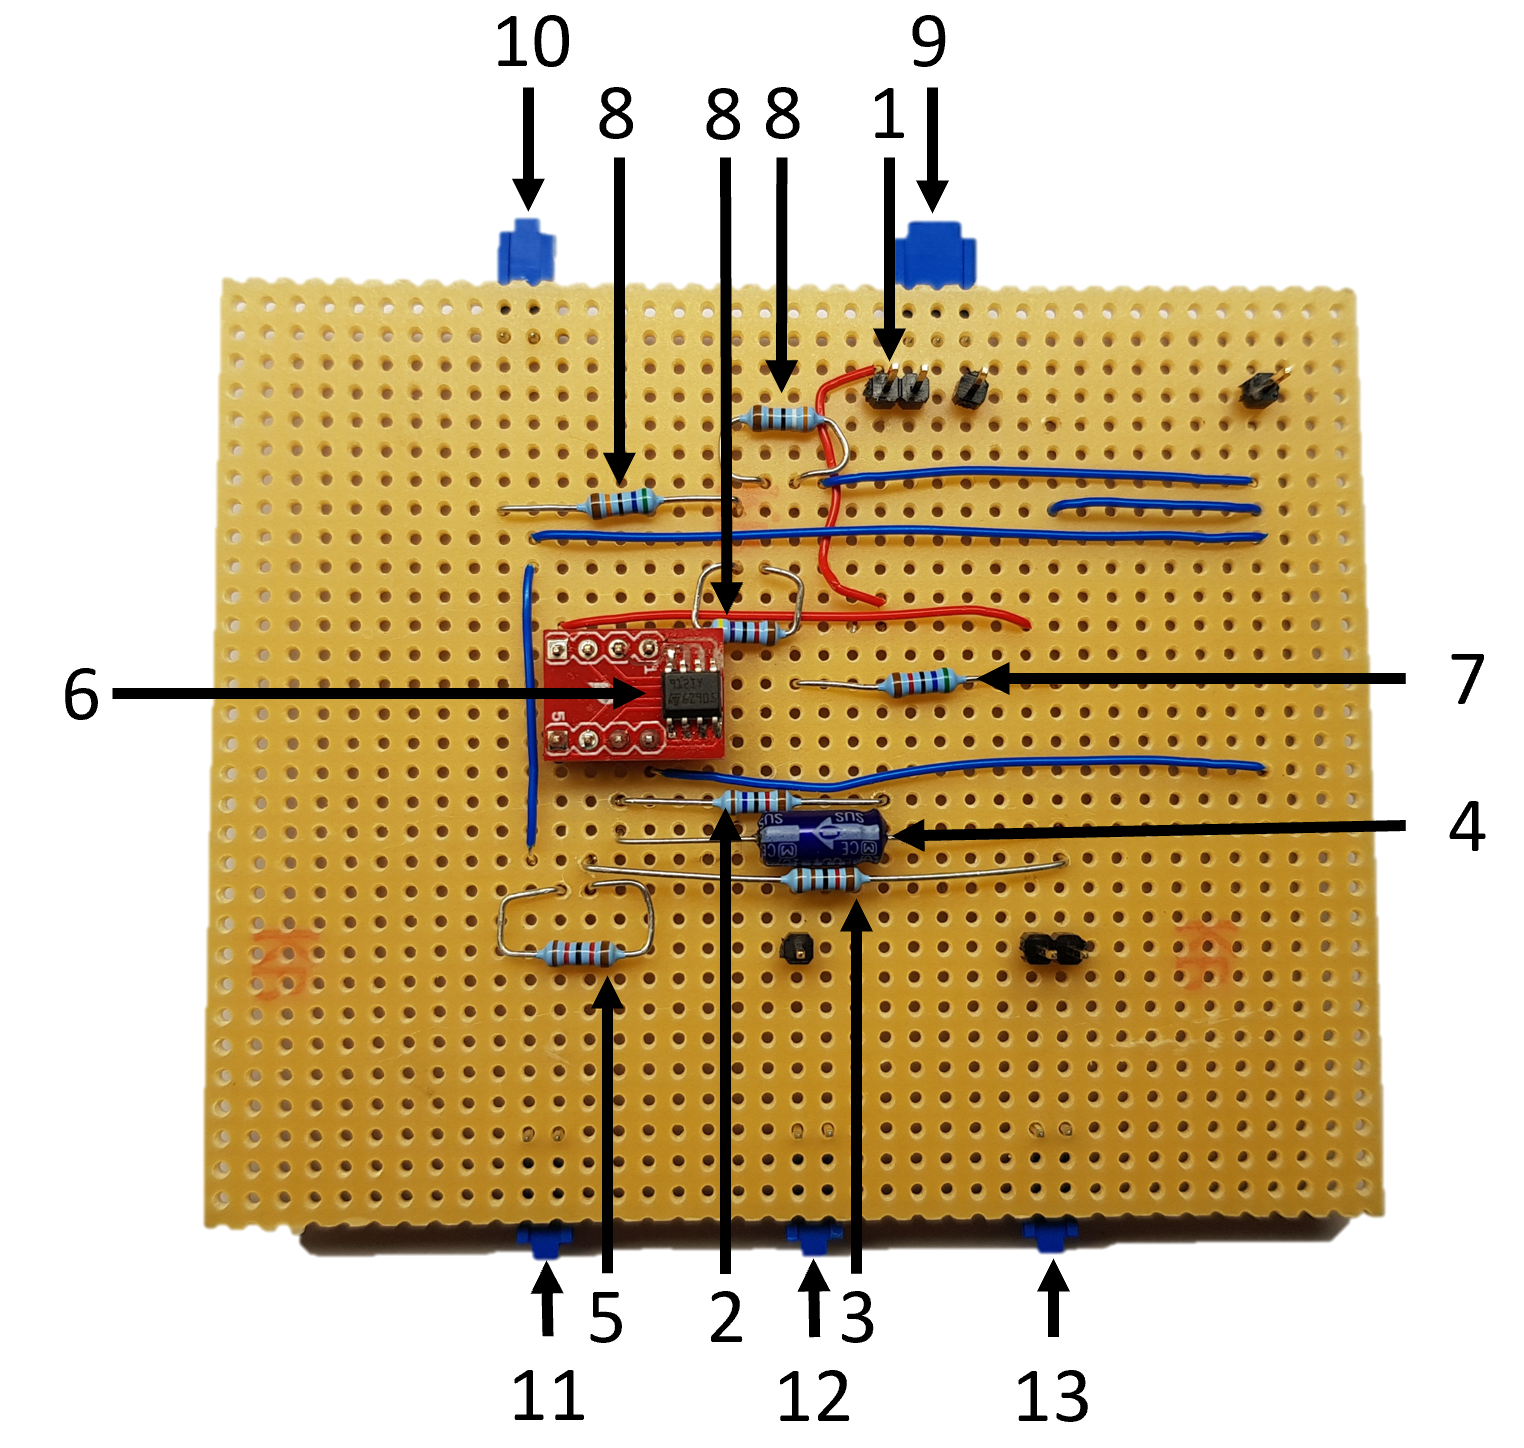
\includegraphics[width=0.7\textwidth]{Laboraufbau.png}	
	\caption{Lochraster Print mit Verstärkerschaltung und Spannungsteiler}\label{fig:Laboraufbau}
\end{figure}

\begin{table}[ht!]
	\centering
	\begin{tabular}{|l|l|}
		\hline
		Nummer & Bauteil                                                             \\ \hline
		1      & PWM-Ausgang Arduino                                                 \\ \hline
		2      & R1 des Filters                                                      \\ \hline
		3      & R2 der Spannungsverstärkungsschaltung                               \\ \hline
		4      & C1 des Filters                                                      \\ \hline
		5      & R3 der Spannungsverstärkungsschaltung                               \\ \hline
		6      & Operationsverstärker TS912                                          \\ \hline
		7      & R4 des Spannungsteilers 											 \\ \hline
		8      & R5 des Spannungsteilers (3 Widerstände seriell)                     \\ \hline
		9      & Freigabe Arduino                                                    \\ \hline
		10     & Eingang Spannungsmessung                                            \\ \hline
		11     & Ausgang Steuerspannung                                              \\ \hline
		12     & Abgriff Spannungsteiler                                             \\ \hline
		13     & Speisespannung Arduino \& Spannungsverstärker                       \\ \hline
	\end{tabular}
	\caption{Beschreibung der Nummern beim Lochraster Print}
	\label{tab:Laboraufbau}
\end{table}

\newpage
\subsubsection*{Filter}
Berechnet wurden die passiven Elemente des Tiefpassfilters mit folgender Grundformel \cite{Tiefpass}:
\begin{equation}
f = \frac{1}{2 \cdot \pi \cdot R_1 \cdot C_1}
\end{equation}


Um die Kapazität des Kondensators oder den Widerstand zu bestimmen, wurde die Grenzfrequenz auf $f$ = \SI{1}{Hz} gesetzt. Ausserdem wählte man die Kapazität auf \SI{10}{\mu F}. Dies ergab einen Widerstand von \SI{16}{\Omega}. 


%Dabei wurde $f$ = \SI{1}{Hz} eingesetzt und so kann die Kapazität oder der Widerstand frei gewählt werden. Für die Kapazität wurde \SI{10}{\mu F} ausgesucht. Somit ergab sich einen Widerstand von \SI{16}{\Omega}. Die Bauteile wurden aufgrund der vorhandenen Bauteile im Labor ausgewählt.


\subsubsection*{Verstärkerschaltung}
Die Verstärkung einer nicht invertierenden Verstärkungsschaltung wird wie folgt berechnet \cite{Verstaerker}:
\begin{equation}\label{eq:Verstärkerschaltung}
V_u = 1 + \frac{R_3}{R_2}
\end{equation}
Um die Ströme klein zu halten, wurden Widerstände von \SI{12}{k\Omega} verwendet. Die Verstärkung muss den Faktor zwei haben, damit die Spannung verdoppelt wird. Daher wurden die beiden Widerstände gleich gross gewählt.


\newpage
\begin{figure}[ht!]  
	\centering 
	\begin{minipage}[t]{.76\textwidth} \centering 
		\centering
		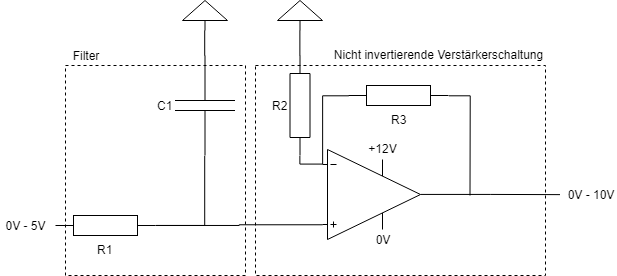
\includegraphics[scale=0.555]{Schema_Verstaerkerschaltung.png}	
		\caption{Schema Verstärkerschaltung}\label{fig:Verstaerkerschaltung}
	\end{minipage}	
	% 
	\begin{minipage}[b]{.23\textwidth}
		\centering
		\begin{tabular}{|l|l|}
			\hline
			R$_1$ & \SI{16}{k\Omega} 	\\ 	\hline
			R$_2$ & \SI{11}{k\Omega} 	\\ 	\hline
			R$_3$ & \SI{12}{k\Omega} 	\\	\hline
			C$_1$ & \SI{10}{\mu F} 		\\	\hline
		\end{tabular}
		\caption{Werte der Bauteile}
		\label{tab:Verstaerkerschaltung}
	\end{minipage}
\end{figure} 



Bei der Verstärkerschaltung wurde die Ausgangsspannung mit einem Duty Cycle von 1 gemessen, was in einer Spannung von \SI{9.885}{V} resultierte. Dies bedeutet, dass der Thyristorsteller nicht voll ausgesteuert wird. Damit man die vollen \SI{10}{V} erhält,wurde bei der Verstärkerschaltung die Verstärkung erhöht. Mit der Formel \ref{eq:Verstaerkungsschaltung_neu} konnte sie neu berechnet werden:

\begin{equation}\label{eq:Verstaerkungsschaltung_neu}
V_u = 1 + \frac{12k\Omega}{11k\Omega} = 2.09
\end{equation}
Mit dem neuen Widerstand $R_2$ wurde am Ausgang  eine Spannung von \SI{10.2}{V} gemessen. Somit kann der gesamte Bereich von 0 - \SI{10}{V} benutzt werden, um den Thyristorsteller anzusteuern.

\subsection{Laboraufbau mit einem Widerstand}
Nach dem Verifizieren der Funktionalität der Spannnungsverstärkungsschaltung konnte mit dem eigentlichen Laboraufbau begonnen werden. Hierbei wurde ein variabler-, dreiphasiger Culatti-Widerstand als Last benutzt. Dieser hat den Vorteil, dass die Last bei allen Phasen symmetrisch sind. Um den Strom kleinzuhalten, wurde ein Widerstand von \SI{150}{\Omega} gewählt. Der Aufbau der Messschaltung ist auf der Abbildung \ref{fig:Messaufbau} ersichtlich.


\begin{figure}[ht!]
	\centering
	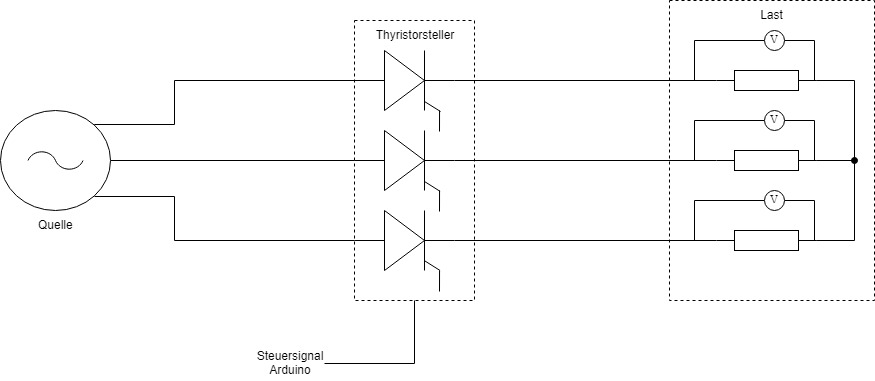
\includegraphics[width=\textwidth]{Messaufbau.png}	
	\caption{Schema Laboraufbau mit einem dreiphasigen Widerstand in Stern geschaltet}\label{fig:Messaufbau}
\end{figure}

Die Last wurde zudem in Dreieck geschaltet, um einen Unterschied von den Strömen und den Spannungen zur Sternschaltung zu erhalten.

\subsection{Laboraufbau mit einer ASM}

Gleich wie beim Laboraufbau des Widerstands wurde bei den Messungen eine Asynchronmaschine als Last in den Stromkreis eingebaut. Die Maschine verhält sich nicht wie der Culatti rein ohmsch, sondern ohmsch-induktiv, das verschiedene Reaktanzen in der Erreger- und Ankerwicklung vorkommen. Daher werden die Spannungen und die Ströme der Maschine anders aussehen als beim Widerstand.  Dabei wurde er in Stern und in Dreieck geschaltet. Ein Vorteil der Maschine, der Marke Lukas Nülle mit einer Leistung von \SI{0.3}{kW}, ist, dass ein integrierter Drehzahlgeber vorhanden ist, um die Drehzahl zu messen. Ein weiterer interessanter Punkt ist, dass beim Wegschalten der Spannung der Motor weiterdreht und so träge auf Veränderungen reagiert.  


\subsection{Arduino}

Als Arduino, welcher den Thyristorsteller ansteuert, wurde ein Arduino Mega2560 verwendet. Dabei wurde der Code mit der Arduinosoftware geschrieben. Mit den verschiedenen I/O Pins können Spannungen bis zu \SI{5}{V} gemessen und ausgegeben werden.
 

\subsubsection*{Phasenanschnittssteuerung mit Arduino}
Die Phasenanschnittsteuerung wird mit der einfachen 0 - \SI{10}{V}-Ansteuerung des Thyristorstellers realisiert. Dabei ist die Ansteuerungskennlinie linear und so entsprechen \SI{10}{V} einem Zündwinkel von 0\textdegree\hspace{0.02cm} und \SI{0}{V} einem Zündwinkel von 180\textdegree. Dieser Ansteuerungsbereich muss auf die 0 bis 255 Werte umgerechnet werden, da der analogWrite()-Bereich des Arduinos so konzipiert ist. Wenn zum Beispiel ein Winkel von 90\textdegree \hspace{0.02cm} erwünscht ist, muss ein Wert von 127 ausgegeben werden.

\subsubsection*{Schwingungspaketsteuerung mit Arduino}
Die Schwingungspaketsteuerung funktioniert mit dem Thyristorsteller nicht so einfach, da dieser nur für den Phasenanschnitt konzipiert ist. Jedoch kann beim Arduino zwischen HIGH und LOW mit einer bestimmten Zeitverzögerung dazwischen umgeschaltet werden. Das Problem, welches dabei auftritt, ist, dass der Thyristorsteller und die Spannungsverstärkerschaltung zusammen eine Zeitverzögerung von \SI{0.2}{s} haben. So schaltet der Sinus verzögert ein und daraus folgt ein sanftes Hochfahren von \SI{0.35}{s}. Ein hartes Zu- und Wegschalten, wie in den Simulationen gezeigt, ist deshalb nicht möglich.


\subsubsection*{Hartes Auf- und Absteuern}
Um das harte Auf- und Absteuern zu implementieren, wurden die beiden vorherigen Verfahren miteinander kombiniert. Dies hat den Grund, dass die Nachteile der beiden vorherigen Verfahren minimiert werden. Anstatt jedoch nur einen Winkel vorzugeben, wurde mit einer for-Schleife die Ansteuerungsspannung und somit der Zündwinkel linear erhöht. Sobald sich die Spannung auf dem Maximum befindet, wartet der Thyristorsteller für \SI{0.2}{s}. In dieser Zeit wird die maximale Spannung ausgegeben. Danach wird mit einer zweiten for-Schleife heruntergefahren. Wenn die minimale Spannung erreicht ist, wartet das Programm \SI{0.1}{s}, bis das nächste Hochfahren beginnt. Dies dient dazu da das Spannungssignal sonst nicht auf \SI{0}{V} geht. Die zwei for-Schleifen befindeen sich in einer dritten for-Schleife, die die Schwingungspaketsteuerung simuliert. Mit ihr kann eingestellt werden, wie oft das Hoch- und Runterfahren durchgeführt wird. Wenn zum Beispiel fünf von zehn Paketen angesteuert werden, fährt das Programm fünfmal hoch- und runter und sperrt die restlichen fünf Pakete. Wie dieser Code aussieht, ist auf der Abbildung \ref{fig:Beispielcode} ersichtlich.
\begin{figure}[ht!]
	\centering
	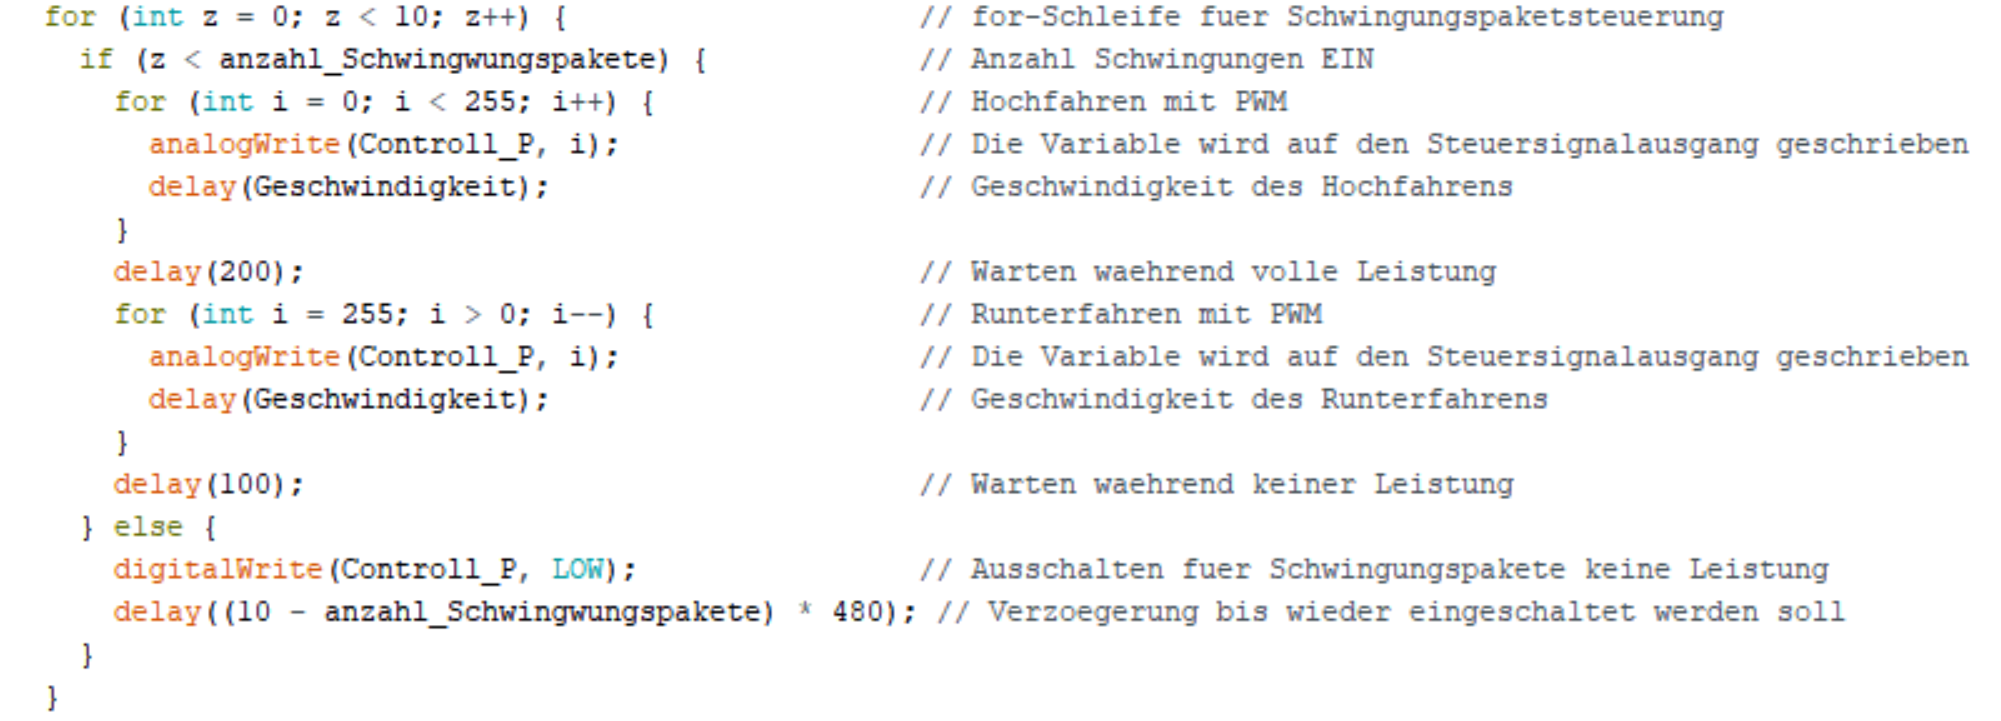
\includegraphics[width=\textwidth]{Beispiel_Code.png}	
	\caption{Hartes Auf-und Absteuern Arduinocode}\label{fig:Beispielcode}
\end{figure}

\subsubsection*{Sanftes Auf- und Absteuern}
Beim sanften Auf- und Absteuern ist die Steigung des Hoch- und Runterfahrens flacher als die beim harten Auf- und Absteuern. Wenn langsamer hoch- und runtergefahren wird, sinken die Werte der harmonischen Oberwellen. Zusätzlich wird nach dem Erreichen der maximalen Spannung eine Verzögerung von \SI{6}{s} eingebaut, damit das Signal \SI{6}{s} auf dem Maximum bleibt. Anschliessend fährt das Programm die Spannung mit der gleichen Steigung wie beim Hochfahren runter und bleibt für \SI{3}{s} auf \SI{0}{V}. Dies kann beliebig oft wiederholt werden.


\subsubsection{Drehzahlmessung für eine Reglerauslegung}
Um die Drehzahl des Asynchronmotors messen und regeln zu können, wurde eine Drehzahlregelung im Arduino programmiert. Dabei wird die Spannung über dem Drehzahlgeber des Asynchronmotors benötigt. Sie beträgt bei der maximalen Drehzahl von \SI{2800}{U/min} \SI{58.8}{V}. Die Spannung ist linear von der Drehzahl abhängig und beträgt so, bei zum Beispiel \SI{1400}{U/min}, \SI{29.4}{V}. Da der Arduino nur eine maximale Spannung von \SI{5}{V} einlesen kann, wird mithilfe eines Spannungsteilers die Spannung des Drehzahlgebers linear reduziert. Mit der Grundformel des Spannungsteilers \ref{eq:Spannungsteiler} und des freien Wählens eines Widerstandes $R_4$ konnte daraus $R_5$ bestimmt werden \cite{Spannungsteiler}:

\begin{equation}\label{eq:Spannungsteiler}
U_2=U_{Ges} \cdot\frac{R_4}{R_4 + R_5} \Longrightarrow 4.94 V = 58.8 V \cdot \frac{56k\Omega}{56k\Omega + R_5}
\end{equation}

Das Resultat des Widerstands $R_5$ ist \SI{611}{k\Omega} und somit konnte die Spannung mit dem Arduino gemessen werden. Mit dem ADC wird sie in 1024 verschiedene Werte aufgeteilt. Der Wert 512 entspricht  einer Spannung von \SI{2.5}{V} \cite{Spannungsmessung}. Danach wird dieser Wert mit den Widerstandswerten des Spannungsteilers auf die Originalspannung zurückgerechnet. Beim Regler wird für den Sollwert ein gewünschter Spannungswert vorgegeben. Anschliessend wird der Istwert vom Sollwert abgezogen, dadurch erhält man die Differenz. Da der Ausgabewert des Arduinos einem Wert zwischen 0 bis 255 entspricht, muss die Differenz umgerechnet werden. Zusätzlich wird ein PI-Regler benötigt, damit eine exakte und schnelle Regelung möglich ist.\\\\
Mit der Formel \ref{eq:digitaler_PI_Regler} wird die Ausgangsspannung eines digitaler PI-Regler berechnet \cite{Quelle_Marco} : 
\begin{equation}\label{eq:digitaler_PI_Regler}
Y(k) = Y(k-1)+ B_0U(k)+B_1U(k-1)
\end{equation}
Wobei $Y$ die Ausgangsspannung, $U$ die Differenzspannung und $k$ der Laufparameter sind. Die Parameter $B_0$ und $B_1$ werden folgendermassen berechnet \cite{PI_Regler}:
\begin{equation}\label{eq:B0}
B_0 = \left(K_p + \frac{K_iT}{2}\right) 
\end{equation}
\begin{equation}\label{eq:B1}
B_1 = -\left(K_p - \frac{K_iT}{2}\right) 
\end{equation}

Danach muss die Spannungsdifferenz von der Ausgangsspannung subtrahiert werden. Das Resultat der Berechnung wird in die 0 bis 255 Werte umgerechnet und mit dem analogWrite() ausgegeben. Die Werte der Ausgangsspannung und der Differenzspannung werden nach der Ausgabe in den Laufparameter $k-1$ geladen. Das Problem mit dem PI-Regler ist, dass der Thyristorsteller und die Spannungsverstärkung eine Verzögerung besitzen. Ausserdem hat der Aurduino keine konstante Abtastrate bei dieser Anwendung. Dadurch ist das Auslegen eines guten Reglers nicht möglich. Der Code für die Drehzahlregelung befindet sich im Anhang im Kapitel \ref{sec:Drehzahlregelung}. Das Blockdiagramm der Formel \ref{eq:digitaler_PI_Regler} ist in Abbildung \ref{fig:PIRegler} ersichtlich.

\begin{figure}[ht!]
	\centering
	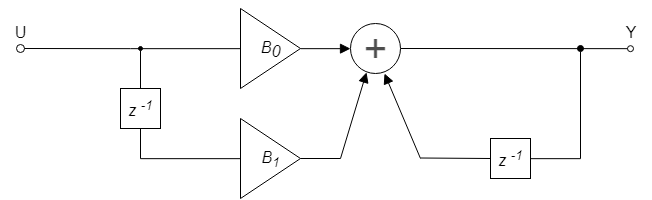
\includegraphics[width=\textwidth]{BlockdiagrammPI.png}	
	\caption{Blockdiagramm eines digitalen PI-Reglers \cite{PI_Regler}}\label{fig:PIRegler}
\end{figure}







